\section{GPA Embeddings}\label{sec:gpa-emb}

This section is devoted to discussing the details of our GPA embeddings.
This will include a discussion of the techniques used to solve the defining equations,
along with a discussion of the coordinates these solutions define.
Subsection~\ref{subsec:extend-level-4} discusses some of the representation theory which led us to 
search for $\Z_n$-like extensions in the first place;
in this respect, we discuss only the details of level 4, but the story at level 3 is essentially the same.

We find our fusion graphs by orbifolding the graphs in Figures 18b and 21b of \cite{g2_graphs}.
These graphs are shown in Figure~\ref{fig:new-graphs}.

\begin{figure}
    \noindent\makebox[\textwidth]{
    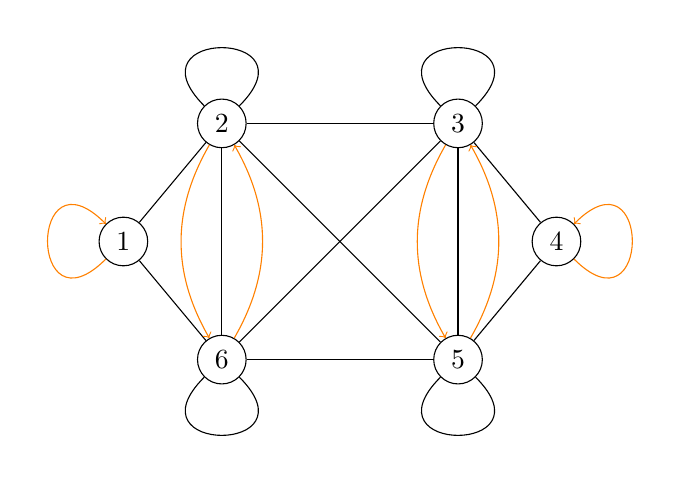
\begin{tikzpicture}[scale=1.0]
        \node[shape=circle,draw=black] (A) at (0,1.5) {1};
        \node[shape=circle,draw=black] (B) at (1.25,3) {2};
        \node[shape=circle,draw=black] (C) at (4.25,3) {3};
        \node[shape=circle,draw=black] (D) at (5.5,1.5) {4};
        \node[shape=circle,draw=black] (E) at (4.25,0) {5};
        \node[shape=circle,draw=black] (F) at (1.25,0) {6};

        % module fusion graph
        \path (B) edge [loop, in=45, out=135, looseness=8] node {} (B);
        \path (C) edge [loop, in=45, out=135, looseness=8] node {} (C);
        \path (E) edge [loop, in=225, out=315, looseness=8] node {} (E);
        \path (F) edge [loop, in=225, out=315, looseness=8] node {} (F);

        \path [-] (A) edge node {} (B);
        \path [-] (A) edge node {} (F);

        \path [-] (B) edge node {} (C);
        \path [-] (B) edge node {} (E);
        \path [-] (B) edge node {} (F);

        \path [-] (C) edge node {} (D);
        \path [-] (C) edge node {} (E);
        \path [-] (C) edge node {} (F);

        \path [-] (D) edge node {} (E);

        \path [-] (E) edge node {} (F);

        % g fusion graph
        \path [->, draw=orange] (A) edge [loop, in=135, out=225, looseness=8] node {} (A);
        \path [->, draw=orange] (D) edge [loop, in=45, out=-45, looseness=8] node {} (D);

        \path [->, draw=orange] (B) edge [bend right] node  {} (F);
        \path [->, draw=orange] (F) edge [bend right] node {} (B);

        \path [->, draw=orange] (C) edge [bend right] node {} (E);
        \path [->, draw=orange] (E) edge [bend right] node {} (C);
    \end{tikzpicture}
    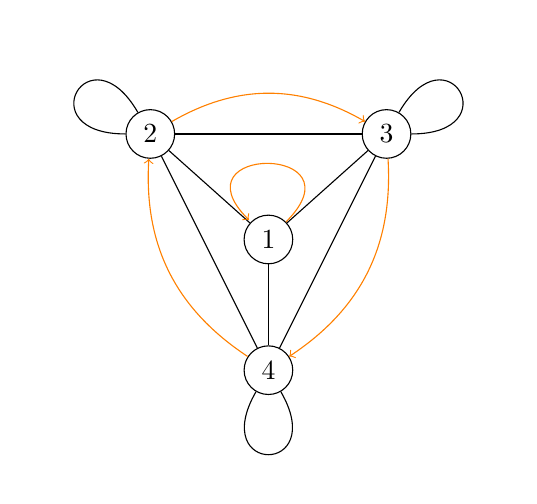
\begin{tikzpicture}[scale=1.0]
        \node[shape=circle,draw=black] (A) at (1.5,1.66) {1};
        \node[shape=circle,draw=black] (B) at (0,3) {2};
        \node[shape=circle,draw=black] (C) at (3,3) {3};
        \node[shape=circle,draw=black] (D) at (1.5,0) {4};
        
        % module fusion graph
        \path (B) edge [loop, in=120, out=180, looseness=10] node {} (B);
        \path (C) edge [loop, in=0, out=60, looseness=10] node {} (C);
        \path (D) edge [loop, in=240, out=300, looseness=10] node {} (D);
        
        \path [-] (D) edge node {} (B);
        \path [-] (B) edge node {} (C);
        \path [-] (C) edge node {} (D);

        \path [-] (A) edge node {} (B);
        \path [-] (A) edge node {} (C);
        \path [-] (A) edge node {} (D);

        % g fusion graph
        \path [->, draw=orange] (B) edge [bend left] node {} (C);
        \path [->, draw=orange] (C) edge [bend left] node {} (D);
        \path [->, draw=orange] (D) edge [bend left] node {} (B);
        \path [->, draw=orange] (A) edge [loop] node {} (A);
    \end{tikzpicture}
    }
    \caption{
        Fusion graphs at level 4 and 3 for $Y_4$ and $Y_3$ (black) and $g_4$ and $g_3$ (orange), respectively. 
        See Figures 21b and 18b, respectively, of \cite{g2_graphs}.
        }
    \label{fig:new-graphs}
\end{figure}


% \begin{figure}
%     \centering
%     \begin{tikzpicture}[scale=1.25]
%         \node[shape=circle,draw=black] (A) at (1.5,1.66) {1};
%         \node[shape=circle,draw=black] (B) at (0,3) {2};
%         \node[shape=circle,draw=black] (C) at (3,3) {3};
%         \node[shape=circle,draw=black] (D) at (1.5,0) {4};
        
%         % module fusion graph
%         \path (B) edge [loop, in=120, out=180, looseness=10] node {} (B);
%         \path (C) edge [loop, in=0, out=60, looseness=10] node {} (C);
%         \path (D) edge [loop, in=240, out=300, looseness=10] node {} (D);
        
%         \path [-] (D) edge node {} (B);
%         \path [-] (B) edge node {} (C);
%         \path [-] (C) edge node {} (D);

%         \path [-] (A) edge node {} (B);
%         \path [-] (A) edge node {} (C);
%         \path [-] (A) edge node {} (D);

%         % g fusion graph
%         \path [->, draw=orange] (B) edge [bend left] node {} (C);
%         \path [->, draw=orange] (C) edge [bend left] node {} (D);
%         \path [->, draw=orange] (D) edge [bend left] node {} (B);
%         \path [->, draw=orange] (A) edge [loop] node {} (A);
%     \end{tikzpicture}
%     \caption{Fusion graphs at level 3 for $Y$ (black) and $g$ (orange). See \cite[Figure 18b]{g2_graphs}.}
%     \label{fig:new-graphs-lvl3}
% \end{figure}


One may give a monoidal functor $F:\GG_2(q_k) \to \GPA(\Gamma)$ by specifying the image of the morphism 
\[
F\left( \skein{skein_figs/trivalent}{0.08} \right) \in \Hom_{\GPA(\Gamma)}(2\to1).
\]
This amounts to giving a list of $M\coloneqq\tr(\Gamma^2\cdot\Gamma)$ complex numbers\footnote{
    We freely switch between using $\Gamma$ to mean the graph itself and the graph's adjacency matrix. }, 
say $a_1,\dots,a_M$. 
Pushing the defining relations of $\GG_2(q_k)$ through $F$, we see that 
these complex numbers satisfy equations in the $a_i$ and $\ol{a_i}$. 
If we assume for now that each $a_i$ is real, then this reduces the system to a collection 
of polynomials in the $a_i$ \footnote{
    This assumption is useful only if it turns out to help us solve the system. 
    In fact, any assumptions we make about this system, if they yield solutions, are in some way valid.
    }.
Once we have the image of the trivalent vertex in hand, we have found an embedding of the planar algebra it generates. 
We can then follow a similar approach to solve for the image
\[
F\left( \skein{skein_figs/dec_tet_5}{0.08} \right) \in \Hom_{\GPA(\Gamma)}(2\to2)
\]
to extend the GPA embedding of $\GG_2(q_k)$ to an embedding of $\DD_k$.
Let us discuss our examples.







\subsection{Level 4 Trivalent Embedding}
We will begin with level 4.
Let $\Gamma_4$ be the graph on the left side of  Figure~\ref{fig:new-graphs}.
Set $q_4 \coloneq e^{2\pi i/48}$.
The following theorem says that we have an embedding of $\ol{\GG_2(q_4)}$ into the GPA on $\Gamma_4$.
A proof of the theorem is extremely straightforward; one must verify some equations.
Why this verification amounts to a proof requires some explanation, and is discussed in detail 
below the theorem.

\begin{theorem}\label{thm:G2-level4-GPA-emb}
    There is a faithful monoidal functor $\ol{F_4}:\ol{\GG_2(q_3)} \hookrightarrow \GPA(\Gamma_4)$.
\end{theorem}
\begin{proof}
    We first construct a monoidal functor $F_4: \GG_2(q_3) \hookrightarrow \GPA(\Gamma_4)$, and then 
    apply Lemma~\ref{lem:simple-unit-unitary}.
    See the Mathematica notebook \verb|/code/level-4/nb-5_verify-triv.nb| for a definition of $F_4$
    and verification of the necessary equations.
\end{proof}

Let us now explain why a proof of the above result amounts to a verification of a system of 
% linear, quadratic, cubic, quartic, and quintic 
equations.
Let 
\[
    (p_1,q_1),\dots,(p_M,q_M)
\]
be the defining basis\footnote{ 
    See the attached Mathematica files for the specific ordering chosen. } 
for $\Hom_{\GPA(\Gamma)}(2\to1)$ ($M=88$ at level 4). Then it must be that 
\[
    F_4 \left( \skein{skein_figs/trivalent}{0.08} \right) = a_1(p_1,q_1)+\cdots+ a_M(p_M,q_M)
\]
for some $a_1,\dots,a_M \in \C$.
The \ref{eq:Bigon} relation, when sent through $F$, becomes the system
\[
    \sum_{i=1}^M a_i(p_i,q_i) \circ \sum_{j=1}^M a_j(q_j,p_j) = k^2 \sum_{e\in E(\Gamma)} (e,e).
\]
This system is quadratic in the $a_i$ since it involves up to two trivalent vertices on either side. 
The \ref{eq:Lolli} and \ref{eq:Rotate} relations therefore determine a system of linear equations; 
the others give cubic, quartic, and quintic equations. 
It is often useful to solve the linear subsystem first and substitute the solution into the quadratic equations. 
For example, when we substitute the linear solution into the (Bigon) and (Tetragon) equations, 
we are able to isolate the following resulting equations:

\begin{equation*}
    a_{8}^2+a_{85}^2 = 4-\sqrt{2}+2 \sqrt{3}-\sqrt{6} 
\end{equation*}

\begin{equation*}
    a_{69}^2+\left(1+\sqrt{\frac{3}{2}}\right) a_{8}^2 = \frac{3+\sqrt{3}+\sqrt{6}}{\sqrt{2}} 
\end{equation*}

\begin{equation*}
    a_{69}^2 \left(\left(2+\sqrt{6}\right) a_{8}^2+\left(2+\sqrt{6}\right)
   a_{85}^2-2 \sqrt{2+\sqrt{3}}\right) = 5+\sqrt{2}+\sqrt{3}+2 \sqrt{6}
\end{equation*}

\begin{equation*}
    2 a_{69}^4+\left(5+2 \sqrt{6}\right)
   a_{85}^4 = \left(3+\sqrt{2}+\sqrt{3}+\sqrt{6}\right) a_{85}^2+3
   \sqrt{6}+\sqrt{3}+2 \sqrt{2}+7 
\end{equation*}


Up to three choices of sign, the solution to this system is
\begin{align*}
    a_{8} & = \sqrt{2+\sqrt{3}-\sqrt{2+\sqrt{3}}} \\
    a_{69} & = \sqrt{\frac{1}{2} \left(-1+\sqrt{2}+\sqrt{3}\right)} \\
    a_{85} & = \sqrt{2+\sqrt{3}-\sqrt{2+\sqrt{3}}} \\
\end{align*}
Similar equations containing $a_{31}$, $a_{55}$, and $a_{63}$ appear as well. 
We may repeat this process and obtain the additional values
\begin{align*}
    a_{31} & = \sqrt{2+\sqrt{3}-\sqrt{2+\sqrt{3}}} \\
    a_{55} & = \sqrt{1-\sqrt{\frac{3}{2}}+\frac{1}{\sqrt{2}}} \\
    a_{63} & = \sqrt{2+\sqrt{3}-\sqrt{2+\sqrt{3}}} \\
\end{align*}
These six values begin a cascade of equation solving. 
They, along with the linear solution, reduce many of the original high-order equations to linear. 
We solve those, then repeat the process until we're forced to confront nonlinearity. 
The nonlinearity we encounter forces us to extract square roots, and ending up with a few degree-16 algebraic numbers. 
For instance,
\[
    a_{10} = \frac{1}{2} \left(\sqrt{1+\sqrt{6-3 \sqrt{3}}}+\sqrt{\sqrt{2+\sqrt{3}}-1}\right).
\]
Up to sign, the coordinates of $F_4 \left( \skein{skein_figs/trivalent}{0.08} \right)$ 
take on the following values:
\begin{align*}
    \alpha_1 & = \sqrt{\frac{1}{2} \left(1+2 \sqrt{2}+\sqrt{3}+\sqrt{6}\right)} \\
    \alpha_2 & = \sqrt{\frac{1}{2} \left(-1+\sqrt{2}+\sqrt{3}\right)} \\
    \alpha_3 & = \sqrt{\frac{3}{2} \left(\sqrt{2+\sqrt{3}}-1\right)} \\
    \alpha_4 & = \sqrt{2+\sqrt{3}-\sqrt{2+\sqrt{3}}} \\
    \alpha_5 & = \sqrt{\frac{1}{2} \left(\sqrt{2+\sqrt{3}}-1\right)}  \\
    \alpha_6 & = \sqrt{\frac{1}{2} \left(\sqrt{3}+\sqrt{2+\sqrt{3}}\right)} \\
    \alpha_7 & = \sqrt{1-\sqrt{\frac{3}{2}}+\frac{1}{\sqrt{2}}}  \\
    \alpha_8 & = \frac{1}{2} \left(\sqrt{1+\sqrt{6-3 \sqrt{3}}}-\sqrt{\sqrt{2+\sqrt{3}}-1}\right) \\
    \alpha_9 & = \frac{1}{2} \left(\sqrt{1+\sqrt{6-3 \sqrt{3}}}+\sqrt{\sqrt{2+\sqrt{3}}-1}\right). \\
\end{align*}
These coordinates of $F_4 \left( \skein{skein_figs/trivalent}{0.08} \right)$ give us a definition of $F_4$.
To show $F_4$ is a monoidal functor amounts to showing that all defining relations of $\GG_2(q)$ are satisfied 
by $F_4 \left( \skein{skein_figs/trivalent}{0.08} \right)$.
This is verified in the Mathematica notebook \verb|/code/level-4/nb-6_verify-g.nb|.


\subsection{Extension of level 4}\label{subsec:extend-level-4}
With our embedding of $\GG_2(q_4)$, i.e. the coordinates of $F_4 \left( \skein{skein_figs/trivalent}{0.08} \right)$, in hand, 
we now know where to find a subcategory of $\GPA(\Gamma_4)$ isomorphic to $\GG_2(q_4)$.
In practice, we are relying on the fact that the free functor gives an embedding 
\[
    \ol{\Rep(U_{q_4}(\gg_2))} \hookrightarrow \ol{\Rep(U_{q_4}(\gg_2))}_{A_4}
\]
which takes the simple $\otimes$-generator $X_4$ to a simple $\otimes$-generator which we denote by $Y_4$.\footnote{
    Simplicity of $Y_4$ may be easily checked using the $X_4$ fusion graph of $\ol{\Rep(U_{q_4}(\gg_2))}$. }
Combine this with the facts that $\ol{\Rep(U_{q_4}(\gg_2))}_{A_4}$ contains a subcategory equivalent to $\Vecc{\Z_2}$,
and that both of the grouplike simples are subobjects of the square of the $\otimes$-generator $Y_4$.
One concludes that $\Hom_{\ol{\Rep(U_{q_4}(\gg_2))}_{A_4}}(Y_4^{\otimes2}\to Y_4^{\otimes2})$ 
contains a projection onto a $\Z_2$-like simple object 
which follows relations analogous to (Recouple) - (decBigon).
Now, to enlarge our copy of $\GG_2(q_4)$ to a $\Z_2$-like extension, we must find 
and element of $\Hom_{\GPA(\Gamma_4)}(2\to 2)$ which captures the behavior of 
the idempotent; the role will be played by $\skein{skein_figs/dec_tet_5}{0.08}$.

To this end, we take an approach similar to the one of the previous subsection.
We may identify $\GG_2(q_4)$ with the trivalent subcategory of $\DD_4$,
and now view $F_4$ as a functor out of this subcategory.
To finish the definition of $F_4$ to be a functor out of $\DD_4$, we must find
the image
\[
    F_4\left( \skein{skein_figs/dec_tet_5}{0.08} \right) \in \Hom_{\GPA(\Gamma_4)}(2\to2)
\]
satisfying the defining relations of $\DD_4$.
We follow a process similar to solving for the image $F_4\left( \skein{skein_figs/trivalent}{0.08} \right)$.
That is, we assume that for some $b_1,\dots,b_N \in \C$ where $N \coloneq \tr(\Gamma^2 \cdot \Gamma^2)$, we have
\[
    F_4\left( \skein{skein_figs/dec_tet_5}{0.08} \right) = \sum_{i=1}^N b_i (p'_i,q'_i).
\]
We may push the relations (Schur 0), (Schur 1), and (decStick) through $F_4$, and obtain a set of equations 
in the $b_i$.
We additionally obtain a large linear system which follows from Lemma~\ref{lem:general-half-braid}.
In the present context, this lemma states that our projection $\skein{skein_figs/dec_tet_5}{0.08}$ 
satisfies the relation
\begin{equation*}
    \skein{/skein_figs/hb_top}{0.11} = \skein{/skein_figs/hb_bottom}{0.15}
\end{equation*}
where the unoriented red strand indicates that the equation 
holds whenever we pick the same orientation for the left and right sides.
Solving these new equations gives us the coordinates of the projection $F_4\left( \skein{skein_figs/dec_tet_5}{0.08} \right)$.


\begin{theorem}\label{thm:D4-GPA-emb}
    There exists an element $P_4 \in\Hom_{\GPA(\Gamma_4)}(2\to 2)$ satisfying the $\Z_2$-like extension relations, 
    with structure constants given by those in Definition~\ref{def:D4}.
\end{theorem}
\begin{proof}
    See the Mathemaica notebook \verb|/code/level-4/nb-6_verify-g.nb| for verification.
\end{proof}




Tables~\ref{tab:lvl-4-proj-coefs-1} and \ref{tab:lvl-4-proj-coefs-2} hold numerical approximations 
of the nonzero projection coordinates.
There are blocks of nonzero coordinates of length 4 and 25. 
These sizes, and the location of the nonzero real coordinates follow naturally when one considers Remark~\ref{rem:Pg-properties}.
The only coordinates of the projection in the GPA which are nonzero are at those basis vectors 
\[
    (i \to\blank\to j, i \to\blank\to j)
\]
where $i\to j$ is a directed edge of the $g$-fusion graph. 
For $i=j=1,4$ there are two possible values for $\blank$; pairing them gives 4 pairs. 
For $i,j\neq 1,4$ there are five possible values for $\blank$; pairing them gives 25 pairs. 
The columns of Tables~\ref{tab:lvl-4-proj-coefs-1} and \ref{tab:lvl-4-proj-coefs-2} give the 
values of the coordinates of the projection, 
with dictionary ordering on the pairs of $\blank$ values. 
That is, the column labeled by $1\to\blank\to1$ shows the coordinates on the ordered basis
\begin{align*}
    (1\to 2 \to1, 1\to 2 \to1) \\
    (1\to 2 \to1, 1\to 3 \to1) \\
    (1\to 3 \to1, 1\to 2 \to1) \\
    (1\to 3 \to1, 1\to 3 \to1) \\
\end{align*}

With this ordering in mind, and recalling that the GPA's dagger operation swaps paths, the conjugate pairs appear where one would expect them.


\begin{table}
    \centering
    \begin{tabular}{|cc|} \hline
        $1\to\blank\to1$ & $4\to\blank\to4$ \\ \hline\hline
        $2.22$  & $2.22$ \\
        $-2.22$ & $-2.22$ \\
        $-2.22$ & $-2.22$ \\
        $2.22$  & $2.22$ \\ \hline
    \end{tabular}
    \caption{The size 4 blocks of nonzero projection coordinates.}
    \label{tab:lvl-4-proj-coefs-1}
\end{table}


\begin{table}
    \noindent\makebox[\textwidth]{
    \begin{tabular}{|cccc|} \hline
        $2\to\blank\to6$                 & $3\to\blank\to5$         & $5\to\blank\to3$           & $6\to\blank\to2$ \\ \hline\hline
        $0.44949$                        & $1$                      & $1$                        & $0.44949$ \\
        $0.474073 - 0.474073 i$          & $0.825482 + 0.564429 i$  & $0.825482 - 0.564429 i$    & $0.474073 + 0.474073 i$ \\
        $-0.123758 - 0.658919 i$         & $0.123758 + 0.658919 i$  & $0.123758 - 0.658919 i$    & $-0.123758 + 0.658919 i$ \\
        $-0.123758 + 0.658919 i$         & -$0.564429 + 0.825482 i$ & -$0.564429 - 0.825482 i$   & $-0.123758 - 0.658919 i$ \\
        $0.474073 + 0.474073 i$          & $0.931852 - 0.362839 i$  & $0.931852 + 0.362839 i$    & $0.474073 - 0.474073 i$ \\
        $0.474073 + 0.474073 i$          & $0.825482 - 0.564429 i$  & $0.825482 + 0.564429 i$    & $0.474073 - 0.474073 i$ \\
        $1$                              & $1$                      & $1$                        & 1 \\
        $0.564429 - 0.825482 i$          & $0.474073 + 0.474073 i$  & $0.474073 - 0.474073 i$    & $0.564429 + 0.825482 i$ \\
        $-0.825482 + 0.564429 i$         & $i$                      & $-i$                       & $-0.825482 - 0.564429 i$ \\ 
        $i$                              & $0.564429 - 0.825482 i$  & $0.564429 + 0.825482 i$    & -i \\
        $-0.123758 + 0.658919 i$         & $0.123758 - 0.658919 i$  & $0.123758 + 0.658919 i$    & $-0.123758 - 0.658919 i$ \\
        $0.564429 + 0.825482 i$          & $0.474073 - 0.474073 i$  & $0.474073 + 0.474073 i$    & $0.564429 - 0.825482 i$ \\
        $1$                              & $0.44949$                & $0.44949$                  & 1 \\
        $-0.931852 - 0.362839 i$         & $0.474073 + 0.474073 i$  & $0.474073 - 0.474073 i$    & $-0.931852 + 0.362839 i$ \\
        $-0.825482 + 0.564429 i$         & $-0.123758 - 0.658919 i$ & $-0.123758 + 0.658919 i$   & $-0.825482 - 0.564429 i$ \\
        $-0.123758 - 0.658919 i$         & -$0.564429 - 0.825482 i$ & -$0.564429 + 0.825482 i$   & $-0.123758 + 0.658919 i$ \\ 
        $-0.825482 - 0.564429 i$         & $-i$                     & $i$                        & $-0.825482 + 0.564429 i$ \\                 
        $-0.931852 + 0.362839 i$         & $0.474073 - 0.474073 i$  & $0.474073 + 0.474073 i$    & $-0.931852 - 0.362839 i$ \\                 
        $1$                              & $1$                      & $1$                        & $1$ \\                 
        $0.564429 - 0.825482 i$          & $-0.825482 - 0.564429 i$ & $-0.825482 + 0.564429 i$   & $0.564429 + 0.825482 i$ \\                 
        $0.474073 - 0.474073 i$          & $0.931852 + 0.362839 i$  & $0.931852 - 0.362839 i$    & $0.474073 + 0.474073 i$ \\                 
        $-i$                             & $0.564429 + 0.825482 i$  & $0.564429 - 0.825482 i$    & $i$ \\                 
        $-0.825482 - 0.564429 i$         & $-0.123758 + 0.658919 i$ & $-0.123758 - 0.658919 i$   & $-0.825482 + 0.564429 i$ \\                 
        $0.564429 + 0.825482 i$          & $-0.825482 + 0.564429 i$ & $-0.825482 - 0.564429 i$   & $0.564429 - 0.825482 i$ \\                 
        $1$                              & $1$                      & $1$                        & $1$ \\ \hline                 
    \end{tabular}
    }
    \caption{The size 25 blocks of nonzero projection coordinates.}
    \label{tab:lvl-4-proj-coefs-2}
\end{table}




As an immediate consequence of Theorems~\ref{thm:G2-level4-GPA-emb} and \ref{thm:D4-GPA-emb} we have the following corollary.

\begin{corollary}\label{cor:D4-unitary}
    The category $\DD_4$ is a nontrivial $\Z_2$-like extension of $\GG_2(q_4)$, 
    and the semisimple quotient $\ol{\DD_4}$ is unitary.
\end{corollary}
\begin{proof}
    We deduce $\DD_4$ is nonzero by its embedding into a nonzero subcategory of $\GPA(\Gamma_4)$.
    Unitarity of its semisimple quotient follows from noting the unitarity of $\GPA(\Gamma_4)$,
    and applying Lemma~\ref{lem:simple-unit-unitary}.
\end{proof}


\begin{corollary}\label{cor:D4-dagger-emb}
    The embedding $\GG_2(q_4) \hookrightarrow \DD_4$ descends to a 
    $\dagger$-embedding $\ol{\GG_2(q_4)} \hookrightarrow \ol{\DD_4}$.
\end{corollary}
\begin{proof}
    Use Lemma~\ref{lem:simple-unit-unitary} again, and compose the induced functor with the functor
    \[
        \DD_4 \onto \ol{\DD_4}
    \]
    onto the semisimple quotient.
\end{proof}
Later, we will take the Karoubi completion of this embedding.
For now, we turn to a discussion of how we obtain the $\DD_4$ structure constants.














\subsection{New Relations at Level 4}
When finding GPA embedding of $\DD_4$, we did not use the relations 
(Swap), (Change of Basis), (decTrigon), (decTetragon), or (decPentagon).
That is, the structure constants in these relations were unknown before exploring our GPA embedding.

In order to discover these new relations,
we hypothesize the form such a relation should take, impose that form, and solve for the structure constants.
For example we would suppose, based the simplicity of $Y_4$ and the invertibility of $g_4$, that an equation of the form
\[
    F_k\left( \skein{/skein_figs/swap_LHS}{0.15} \right) = \omega F_k\left( \skein{/skein_figs/swap_RHS}{0.15} \right)
\]
holds, for some $\omega$.
With our explicit GPA embeddings of the projection in hand, discovering what $\omega$ is becomes a matter of solving
a system of linear equations for one variable.

Discovering the (decTrigon) structure constants is similarly reduced to solving a system of linear equations of the form
\[
F_k\left( \skein{/skein_figs/dec_trigon_LHS}{0.1} \right)= 
        t_1 F_k\left( \skein{/skein_figs/trivalent}{0.1} \right) 
        + t_2 F_k\left( \skein{/skein_figs/triv_rightUp}{0.1} \right)
\]
for $t_1$ and $t_2$.
In practice, the hom-spaces in the GPAs we used were sufficiently large 
making solving all of these equations fairly straightforward.














\subsection{Level 3 Trivalent Embedding}
We now tell a similar story, but at level 3.
However, for the trivalent coefficients we use numerical approximations here, 
and relegate the actual numbers to the attached Mathematica files.
We were unable to find presentable representations of the GPA-embedding coordinates or structure constants.
The coordinates for the trivalent GPA embedding were algebraic numbers of degree 12 or 24.
Even worse, the structure constants for the relations (Change of Basis), (decTrigon), (decTetragon), and (decPentagon) 
are all of the form
\[
    g_1 + g_2 \alpha^2 + g_3 q_3 + g_4 \alpha^2 q_3
\]
where $g_i\in \Q(q_3+q_3^{-1})$, the maximal real subfield of $\Q(q_3)$, 
and $\alpha$ is an algebraic number of degree 24 which appears as a coordinate of 
$F_3 \left( \skein{skein_figs/trivalent}{0.08} \right)$.
For the relations (Change of Basis) and (decTrigon), the power basis coordinates of the $g_i$ are lowest form rational numbers 
whose numerators have one or two digits.
For (decTetrgon), the numerators and denominators of the power basis coordinates of the $g_i$ have around 10 digits on average.
In the (decPentagon) relation, this digit count explodes to around 135.

Let $\Gamma_3$ be the graph given in the right side of Figure~\ref{fig:new-graphs}.
Set $q_3 \coloneq e^{2\pi i/42}$.
The following result gives us a GPA embedding of $\ol{\GG_2(q_3)}$.

\begin{theorem}\label{thm:G2-level3-GPA-emb}
    There is a faithful monoidal functor $\ol{F_3}: \ol{\GG_2(q_3)} \to \GPA(\Gamma_3)$.
\end{theorem}
\begin{proof}
    Similar to Theorem~\ref{thm:G2-level4-GPA-emb}.
    See the Mathematica notebook \verb|/code/level-4/nb-6_verify-g.nb| for 
    verification of the necessary equations.
\end{proof}

Despite the more difficult numbers, we are able to recover some of the structure of the fusion graph in the GPA coordinates.
Recall that the defining bases for the spaces 
\[
    \Hom_{\GPA(\Gamma)}(m\to n)
\]
are given in terms of pairs of paths. 
The (undirected) graphs we are using have at most a single edge between any two vertices. 
Hence an edge is equivalent to a pair of vertices, and a path is equivalent to an ordered tuple of vertices. 
For example, the path
\[
    p = v_1 \longrightarrow v_2 \longrightarrow v_3
\]
is equivalent to the ordered triple $(v_1,v_2,v_3)$. 
Which paths $q$ pair validly with $p$ to form a basis element of the $2\to 1$ hom-space of a GPA? 
Well, by definition, $q$ must be parallel to $p$; i.e. the sources and targets of $p$ and $q$ must coincide. 
It follows that the only valid pairing for such $p$ is
\[
    q = v_1 \longrightarrow v_3,
\]
which may also be represented as $(v_1,v_3)$. 
So the only $2\to 1$ basis element which $p$ appears in is
\[
    \big( (v_1,v_2,v_3), (v_1,v_3) \big).
\]
But the parallel condition defining basis elements makes including $(v_1,v_3)$ redundant; 
we might just as well have called the basis element by 
\[
    (v_1,v_2,v_3).
\]
This is how we refer to $2\to 1$ GPA basis elements. 
Indeed, in Table~\ref{tab:lvl-3-triv-coefs}, the first two columns combine to specify which basis elements are being specified, 
and the third column gives the approximate coordinate of the trivalent embedding on that basis element. 
For example, the first row of Table~\ref{tab:lvl-3-triv-coefs} tells us that the 
coordinate of the $(2,2,2)$ basis element is approximately $1.08393$; 
the second row tells us that the coordinate of the $(4,2,3)$ basis element is approximately $0.619371$. 

Paths of the form $(i,j,i)$, $(i,i,j)$, or $(i,j,j)$ for $i,j\neq1$ require a bit more care to describe. 
There is nontrivial interplay with the graph symmetry swapping vertices 2 and 4. 
When these two vertices are swapped, a path whose coordinate has absolute value $0.155691$ is sent to 
one whose coordinate has absolute value $1.69414$. 
The nine paths whose coordinates have absolute value $0.155691$ are:
\[
    (2,3,3),\hspace{0.2em} (3,3,2),\hspace{0.2em} (3,2,3),\hspace{0.2em} (2,4,2),\hspace{0.2em} (4,3,4),\hspace{0.2em} (2,2,4),\hspace{0.2em} (3,4,4),\hspace{0.2em} (4,2,2),\hspace{0.2em} (4,4,3) 
\]
One may use the symmetry $2 \xleftrightarrow{} 4$ to find the rest of the coordinates.






\begin{table}
    \centering
    \begin{tabular}{|cc|c|} \hline
        Vertex Path & Conditions & Coefficient \\ \hline\hline
        $(i,i,i)$ &  $i\neq1$ & 1.08393 \\[10pt]  \hline
        $(i,j,k)$ &  $\{i,j,k\}=\{2,3,4\}$   & 0.619371 \\[10pt] \hline
        $(i,1,k)$ &  $i,k\neq 1$, $i\neq k$ & 1.69414 \\[10pt] \hline
        $(i,1,i)$ &  $i\neq 1$   & 0.861006 \\[10pt] \hline
        $(i,i,1)$ or $(1,i,i)$ &  $i\neq1$   & 0.967919 \\[10pt] \hline
    \end{tabular}
    \caption{Level 3 trivalent embedding coefficients.}
    \label{tab:lvl-3-triv-coefs}
\end{table}



\subsection{Extension of level 3}
\begin{theorem}\label{thm:D3-GPA-emb}
    There exists an element $P_3  \in\Hom_{\GPA(\Gamma_3)}(2\to 2)$ satisfying the $\Z_2$-like extension relations, 
    with structure constants given in the Mathematica notebook \verb|/code/level-3/nb-6_verify-g.nb|.
\end{theorem}
\begin{proof}
    This result is again proved by direct verification of the required equations.
    See the Mathematica notebook \verb|/code/level-3/nb-6_verify-g.nb|.
\end{proof}

Similarly to the level 4 case, Theorems~\ref{thm:G2-level3-GPA-emb} and \ref{thm:D3-GPA-emb}
imply nontriviality and unitarity of $\ol{\DD_3}$.

\begin{corollary}\label{cor:D3-unitary}
    The category $\DD_3$ is a nontrivial $\Z_3$-like extension of $\GG_2(q_3)$, 
    and the semisimple quotient $\ol{\DD_3}$ is unitary.
\end{corollary}


\begin{corollary}\label{cor:D3-dagger-emb}
    The embedding $\GG_2(q_3) \hookrightarrow \DD_3$ descends to a 
    $\dagger$-embedding $\ol{\GG_2(q_3)} \hookrightarrow \ol{\DD_3}$.
\end{corollary}




\begin{table}
    \noindent\makebox[\textwidth]{
    \begin{tabular}{|cccc|} \hline
        $1\to\blank\to1$                    & $2\to\blank\to4$                  & $3\to\blank\to2$               & $4\to\blank\to3$ \\ \hline\hline
        $1.26376$              & $0.791288$                & $0.791288 $              & $0.791288$ \\
        $-0.631881-1.09445 i$   & $0.567622 - 0.684904 i$   & $0.876955 + 0.149123 i$  & $0.674406 + 0.580055 i$ \\
        $-0.631881+1.09445 i$   & $0.674406 + 0.580055 i$   & $0.567622 - 0.684904 i$  & $0.876955 + 0.149123 i$ \\
        $-0.631881+1.09445 i$   & $-0.876955 - 0.149123 i$  & $-0.674406 - 0.580055 i$ & $0.567622 - 0.684904 i$ \\
        $1.26376$               & $0.567622 + 0.684904 i$   & $0.876955 - 0.149123 i$ & $0.674406 - 0.580055 i$ \\
        $-0.631881-1.09445 i$   & $1$                       & $1$                      & $1$ \\
        $-0.631881-1.09445 i$   & $-0.0182917 + 0.999833 i$ & $0.5 - 0.866025 i$       & $0.856735 - 0.515757 i$ \\
        $-0.631881+1.09445i$    & $-0.5 - 0.866025 i$       & $-0.856735 - 0.515757 i$ & $-0.0182917 - 0.999833 i$ \\
        $1.26376$               & $0.674406 - 0.580055 i$   & $0.567622 + 0.684904 i$  & $0.876955 - 0.149123 i$ \\ 
                              & $-0.0182917 - 0.999833 i$ & $0.5 + 0.866025 i$       & $0.856735 + 0.515757 i$ \\
                              & $1$                       & $1$                      & $1$ \\
                              & $-0.856735 + 0.515757 i$  & $0.0182917 - 0.999833 i$ & $0.5 - 0.866025 i$ \\
                              & $-0.876955 + 0.149123 i$  & $-0.674406 + 0.580055 i$ & $0.567622 + 0.684904 i$ \\
                              & $-0.5 + 0.866025 i$       & $-0.856735 + 0.515757 i$ & $-0.0182917 + 0.999833 i$ \\
                              & $-0.856735 - 0.515757 i$  & $0.0182917 + 0.999833 i$ & $0.5 + 0.866025 i$ \\
                              & $1$                       & $1$                      & $1$ \\ \hline
    \end{tabular}
    }
    \caption{Level 3 projection embedding coefficients.}
    \label{tab:lvl-3-proj-coefs}
\end{table}





